\documentclass[11pt,a4paper]{article}

% --- Packages ---
\usepackage[utf8]{inputenc}
\usepackage[T1]{fontenc}
\usepackage[margin=1in]{geometry}
\usepackage{amsmath,amssymb,amsthm}
\usepackage{hyperref}
\usepackage{xcolor}
\usepackage{graphicx}
\usepackage{enumitem}
\usepackage{booktabs}
\usepackage{tabularx}
\usepackage{fancyhdr}
\usepackage{cite}
\usepackage{float}
\usepackage{caption}
\usepackage{listings}
\usepackage{tikz}
\usetikzlibrary{arrows.meta, positioning, shapes, fit, backgrounds, matrix}

% --- Metadata ---
\title{\textbf{CRABS: Cryptographic Attribute-Based State Machines (Extended)}\\[4pt]
\large \textit{A Unified Protocol for Self-Sovereign Authorization with OT/CRDT Hybrid Convergence}}
\author{Victor J. Morrow\\[4pt]
\textit{Prometheus}\\[4pt]
\texttt{victor.j.morrow@gmail.com}}
\date{}

% --- Styling ---
\pagestyle{fancy}
\fancyhf{}
\fancyhead[L]{\small CRABS: Cryptographic Attribute-Based State Machines (Extended)}
\fancyhead[R]{\small Victor J. Morrow}
\fancyfoot[C]{\thepage}
\renewcommand{\headrulewidth}{0.4pt}

\definecolor{codebg}{rgb}{0.95,0.95,0.95}
\lstset{
  basicstyle=\ttfamily\small,
  backgroundcolor=\color{codebg},
  frame=single,
  breaklines=true,
  aboveskip=8pt,
  belowskip=8pt,
  tabsize=2,
  showstringspaces=false
}

% --- Commands ---
\newcommand{\crab}{\textsc{CRABS}}
\newcommand{\abe}{\textsc{ABE}}
\newcommand{\crdt}{\textsc{CRDT}}
\newcommand{\ot}{\textsc{OT}}
\newcommand{\ecdsa}{\textsc{ECDSA}}
\newcommand{\msk}{\textsc{MSK}}
\newcommand{\mpk}{\textsc{MPK}}

\begin{document}

\maketitle

\begin{center}
\rule{0.5\textwidth}{0.4pt}
\end{center}

\begin{abstract}
\noindent We present \textbf{CRABS}, a protocol that unifies Attribute-Based Encryption (ABE), Conflict-free Replicated Data Types (CRDTs), and Operational Transformation (OT) into a single framework for decentralized, self-sovereign authorization. CRABS treats \textbf{attributes as state}---the set of all users and their attributes is the state of a protocol-governed machine, eliminating the central authority problem inherent in traditional ABE. We extend the protocol with \textbf{OT/CRDT hybrid types} that combine the expressiveness of operational transformation with the convergence guarantees of CRDTs, enabling move, swap, reorder, and intent-preserving merge operations on ordered data structures. We introduce \textbf{threshold triggers}---state-conditional attribute issuance that bridges dynamic state changes with ABE decryption capabilities. The protocol supports \textbf{cryptographic agility} through a pluggable signature scheme interface, \textbf{idempotent operations} through declarative dedup specifications, and \textbf{tombstone management} through a unified compaction framework. We describe the protocol's architecture, algorithms, security properties, and limitations, and discuss applications to decentralized organizations, collaborative content platforms, and self-sovereign identity systems.
\end{abstract}

% ======================================================================
\section{Introduction}
% ======================================================================

\subsection{Motivation}

Attribute-Based Encryption (ABE)~\cite{sahai2005fuzzy} provides fine-grained access control by associating decryption keys with sets of attributes. A ciphertext encrypted under the policy \texttt{(role: manager AND department: engineering)} can be decrypted by any user whose key carries those attributes---without the encryptor knowing the recipients in advance. This makes ABE naturally suited for decentralized, broadcast-style encryption.

However, ABE suffers from a fundamental operational limitation: \textbf{only a central authority holding the Master Secret Key (MSK) can issue, modify, or revoke attributes}. This creates a single point of trust, hinders self-sovereign identity, and makes dynamic attribute management impractical. A user who changes departments, gets married, or is promoted must obtain an entirely new key from the authority. There is no audit trail for attribute changes, and users cannot self-assert attributes without going through the central authority.

Concurrently, Conflict-free Replicated Data Types (CRDTs)~\cite{shapiro2011crdt} have emerged as a foundation for decentralized state convergence. CRDTs allow multiple replicas to be updated independently and merged without conflicts, making them ideal for peer-to-peer systems. However, basic CRDTs have \textbf{limited expressiveness}---they support counters, sets, and registers, but cannot represent ordered structures with move, swap, or reorder operations. Operational Transformation (OT)~\cite{ellis1989ot} provides intent-preserving transformations for collaborative editing, but traditionally requires a central sequencer.

Raph Levien's work on the synthesis of OT and CRDTs~\cite{levien2016synthesis} demonstrates that the transform function---not the sequencer---is the heart of the system. By carrying a transform function with each operation and maintaining a causal context, data structures can be both \textbf{convergent} (CRDT property) and \textbf{expressive} (OT property).

\subsection{Our Approach}

We present \textbf{CRABS} (Cryptographic Role-based Attribute-gated Blockchain-like State machines), a protocol that unifies these threads into a single framework. The key insight is:

\begin{quote}
\textbf{Attributes are not keys. Attributes are state.}
\end{quote}

In CRABS, the set of all users and their attributes is the state of a \textbf{protocol state machine}---the Attribute Machine. Changing an attribute (granting a role, verifying an identity, self-asserting a phone number) is a \textbf{state transition} governed by the same protocol rules as any other operation. ABE keys issued to users are \textbf{derived from the current state} and become invalid when the state changes.

We extend this foundation with:

\begin{enumerate}[leftmargin=*,label={\arabic*.}]
    \item \textbf{OT/CRDT Hybrid Types}: Data types that combine the expressiveness of operational transformation with the convergence guarantees of CRDTs, supporting insert, delete, move, swap, and intent-preserving merge on ordered structures.
    \item \textbf{Threshold Triggers}: State-conditional attribute issuance---when a state condition becomes true (e.g., \texttt{video.flags >= 10}), the protocol automatically issues temporary attributes to specified roles, enabling state-conditional decryption.
    \item \textbf{Cryptographic Agility}: A pluggable signature scheme interface supporting ECDSA, Ed25519, BLS, Dilithium, and future schemes through a unified VTable abstraction.
    \item \textbf{Idempotent Operations}: Declarative dedup specifications (\texttt{PER\_USER}, \texttt{GLOBAL}, \texttt{CUSTOM}) that prevent the same logical action from being performed twice, with CRDT-safe convergence.
    \item \textbf{Unified Tombstone Compaction}: A framework for managing tombstone growth across all CRDT types, with vector-clock-based safety checks and configurable compaction strategies.
\end{enumerate}

\subsection{Contributions}

This paper makes the following contributions:

\begin{enumerate}[leftmargin=*,label={\arabic*.}]
    \item \textbf{The CRABS protocol}---A unified architecture combining ABE, CRDTs, OT, and protocol state machines for self-sovereign attribute management.
    \item \textbf{The Attribute Machine}---A state machine whose state \textit{is} the attribute universe, eliminating the central authority problem.
    \item \textbf{OT/CRDT Hybrid Types}---A family of data types that combine OT expressiveness with CRDT convergence, with a formal transform matrix and position map implementation.
    \item \textbf{Threshold Triggers}---A mechanism for state-conditional attribute issuance, bridging dynamic state changes with ABE decryption.
    \item \textbf{Pluggable Cryptographic Agility}---A VTable-based abstraction for signature schemes, enabling multi-scheme support and graceful migration.
    \item \textbf{Unified Compaction Framework}---A tombstone management system applicable to all CRDT types, with safety guarantees based on vector clock synchronization.
\end{enumerate}

% ======================================================================
\section{Related Work}
% ======================================================================

\subsection{Attribute-Based Encryption}

ABE was introduced by Sahai and Waters~\cite{sahai2005fuzzy} as ``Fuzzy Identity-Based Encryption.'' Goyal et al.~\cite{goyal2006abe} formalized Key-Policy ABE (KP-ABE), and Bethencourt, Sahai, and Waters~\cite{bethencourt2007cpabe} introduced Ciphertext-Policy ABE (CP-ABE), the variant used in CRABS. Multi-authority ABE~\cite{chase2007multi} and decentralized ABE~\cite{lewko2011decentralizing} distribute trust across multiple authorities but still require each authority to manage its own attribute domain. CRABS is, to our knowledge, the first system to treat attributes as protocol-governed state rather than static cryptographic material.

\subsection{Operational Transformation and CRDTs}

Operational Transformation (OT) was pioneered by Ellis and Gibbs~\cite{ellis1989ot} for collaborative text editing. The Jupiter system~\cite{nichols1995jupiter} introduced a central server for operation ordering. Raph Levien's work~\cite{levien2016synthesis} demonstrated that OT and CRDTs can be synthesized: operations carry transform functions that adjust them against concurrent operations, achieving convergence without a central sequencer.

CRDTs were formalized by Shapiro et al.~\cite{shapiro2011crdt}. Types include G-Counters (grow-only counters), PN-Counters, OR-Sets (observed-remove sets), LWW-Registers (last-writer-wins registers), and RGA (Replicated Growable Arrays)~\cite{levien2016rga}. CRABS extends these with OT/CRDT hybrids that support move, swap, reorder, and intent-preserving merge.

\subsection{Protocol State Machines and Session Types}

Protocol state machines, also known as typestate~\cite{deline2004typestate} or session types~\cite{honda1998session}, specify valid sequences of operations on a resource. CRABS extends typestate to a decentralized, CRDT-based setting where multiple participants can observe and verify protocol compliance. The resource locking protocol in CRABS is a direct application of typestate to resource scarcity.

\subsection{Self-Sovereign Identity}

Self-Sovereign Identity (SSI)~\cite{allen2016ssi} is a paradigm where individuals control their own digital identities without relying on central authorities. Verifiable Credentials (VCs) and Decentralized Identifiers (DIDs) are key building blocks. CRABS's Attribute Machine provides a cryptographic foundation for SSI, where attributes are self-asserted or verified by peers, and all changes are recorded in an auditable transition log.

\subsection{Capability-Based Security}

Capability systems~\cite{dennis1966capability} grant access based on possession of a capability token rather than identity. CRABS's capability vault---where ABE-encrypted ECDSA signing keys serve as capabilities---applies this principle to the attribute-based setting.

% ======================================================================
\section{The CRABS Protocol}
% ======================================================================

\subsection{Architecture Overview}

CRABS consists of three layers, shown in Figure~\ref{fig:architecture}.

\begin{figure}[H]
\centering
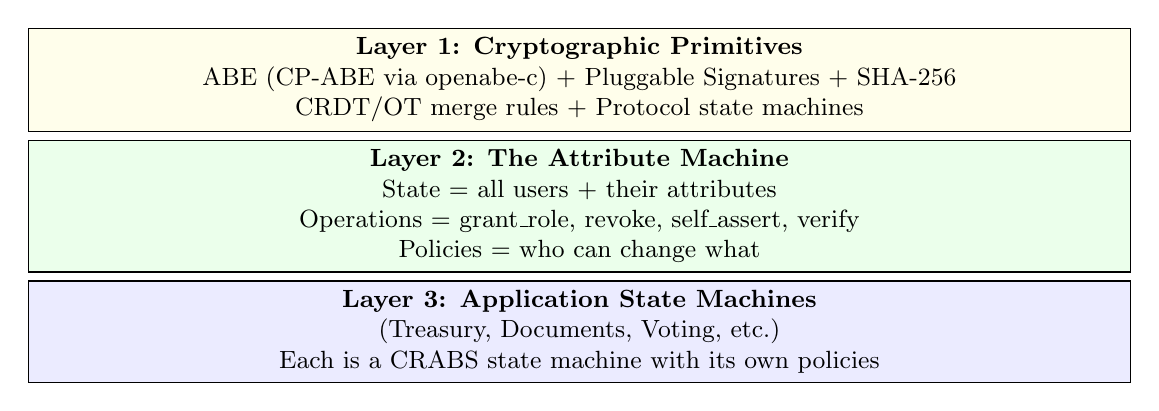
\begin{tikzpicture}[
    box/.style={draw, rectangle, minimum width=14cm, minimum height=1.2cm, align=center, font=\small},
]
    \node[box, fill=blue!8] (l3) {\textbf{Layer 3: Application State Machines}\\(Treasury, Documents, Voting, etc.)\\Each is a CRABS state machine with its own policies};
    \node[box, fill=green!8, above=0.1cm of l3] (l2) {\textbf{Layer 2: The Attribute Machine}\\State = all users + their attributes\\Operations = grant\_role, revoke, self\_assert, verify\\Policies = who can change what};
    \node[box, fill=yellow!8, above=0.1cm of l2] (l1) {\textbf{Layer 1: Cryptographic Primitives}\\ABE (CP-ABE via openabe-c) + Pluggable Signatures + SHA-256\\CRDT/OT merge rules + Protocol state machines};
\end{tikzpicture}
\caption{The three-layer CRABS architecture.}
\label{fig:architecture}
\end{figure}

The Attribute Machine is the foundation. Application machines reference its state for authorization decisions. All machines follow the same protocol.

\subsection{Data Model}

The state of a CRABS machine is a \textbf{bag of typed data items}:

\begin{lstlisting}
State = {
    version: uint64,
    items: {
        "<name>": DataItem,
        ...
    },
    policies: {
        "<operation>": "<abe_policy_expression>",
        ...
    },
    lock_manager: LockManager,
    triggers: { ... },
    log: TransitionLog,
    config: MachineConfig
}
\end{lstlisting}

Each data item has a type, a CRDT merge strategy, a protocol state (for resource types), and a set of invariants. The type system includes basic CRDTs (counters, sets, registers, RGA) and OT/CRDT hybrids (ordered sets, rich documents, trees).

\subsection{The Attribute Machine}

The Attribute Machine is a CRABS state machine whose state \textit{is} the set of all users and their attributes:

\begin{lstlisting}
AttributeMachine State = {
    users: {
        "alice": {
            attributes: {
                role: "writer",
                dept: "engineering",
                phone: "555-0123",          // Self-asserted
                name: "Alice Smith"         // Verified by HR
            },
            keys: { ... },                  // Multiple signature keys
            status: "active",
            key_version: 42
        }
    },
    policies: {
        "grant_role":      "role:admin",
        "revoke_role":     "role:admin",
        "verify_identity": "role:admin OR role:verifier",
        "self_assert":     "role:member",
        "change_policy":   "role:admin AND weight >= 3"
    },
    triggers: { ... }
}
\end{lstlisting}

\textbf{Key insight:} The Attribute Machine follows the \textit{same protocol} as any other CRABS machine. There is no privileged ``authority''---only protocol rules.

\subsection{Key Derivation and Versioning}

ABE keys are derived from the current state of the Attribute Machine:

\begin{lstlisting}
KeyEnvelope = {
    user_id: "alice",
    state_version: 42,
    attributes_hash: SHA256(alice_attrs),
    sk_abe: ABE_keygen(MSK, "role:writer|dept:engineering|...")
}
\end{lstlisting}

When attributes change, the state version increments, and users request key refreshes. Old keys are automatically invalidated by version mismatch.

% ======================================================================
\section{OT/CRDT Hybrid Types}
% ======================================================================

\subsection{Motivation}

Basic CRDTs support counters, sets, and registers but cannot represent ordered structures with move, swap, or reorder operations. For example, an OR-Set cannot express ``move element from position 5 to position 2''---it can only add and remove. RGA supports insert and delete at positions but not move or swap.

OT/CRDT hybrid types extend CRDTs with the expressiveness of operational transformation while preserving convergence guarantees.

\subsection{Coordinate Spaces}

Every OT/CRDT hybrid type maintains two coordinate spaces:

\begin{lstlisting}
Internal coordinates:
    The full structure, including deleted elements.
Visible coordinates:
    What users see and reference in operations.
\end{lstlisting}

The mapping between spaces is maintained by a \textbf{position map}---a balanced BST that tracks all deleted and inserted positions:

\begin{lstlisting}
xi(map, internal_pos) -> visible_pos       // Internal -> visible
xi_inv(map, visible_pos) -> internal_pos   // Visible -> internal
\end{lstlisting}

\subsection{The Transform Matrix}

Every OT/CRDT type defines a transform matrix specifying how each operation type transforms against every other:

\vspace{6pt}
\begin{table}[H]
\centering
\renewcommand{\arraystretch}{1.3}
\begin{tabular}{l|llll}
\multicolumn{1}{c}{} & \textbf{INSERT($j$)} & \textbf{DELETE($j$)} & \textbf{MOVE($j \to k$)} & \textbf{SWAP($j,k$)} \\
\midrule
\textbf{INSERT($i$)}       & priority compare & shift\_left if $i>j$  & shift\_left if $i>j$     & shift\_left if $i>\min(j,k)$ \\
\textbf{DELETE($i$)}       & shift\_right if $i\geq j$ & no\_conflict  & adjust     & adjust \\
\textbf{MOVE($i\to l$)}    & shift\_right if $i\geq j$ & shift\_left if $i>j$ & composite  & composite \\
\textbf{SWAP($i_1,i_2$)}   & shift\_right if $i_1\geq j$ & shift\_left if $i_1>j$ & composite  & composite \\
\end{tabular}
\caption{Transform matrix for OT/CRDT hybrid types. Rows are incoming operations, columns are existing operations. Cells describe how the incoming operation is transformed.}
\label{tab:transform}
\end{table}

\subsection{Priority-Based Deterministic Ordering}

Concurrent inserts at the same position are ordered deterministically by priority:

\[
\text{priority} = (\text{node\_timestamp} \ll 48) \mid (\text{node\_id\_hash} \mathbin{\&} \text{0xFFFF})
\]

Higher priority inserts before lower priority at the same position. Priority is unique across all nodes (node\_id ensures uniqueness).

\subsection{The Merge Algorithm}

\begin{lstlisting}
Algorithm: OT_CRDT_MERGE

Input:
  item_a -- Local replica
  item_b -- Remote replica

1. new_ops = item_b.op_log \ item_a.op_log
2. merged = copy(item_a)
3. for each op in new_ops:
4.     for each existing_op in merged.op_log:
5.         if concurrent(existing_op, op):
6.             op = TRANSFORM(op, existing_op)
7.             merged.op_log[i] = TRANSFORM(existing_op, op)
8.     APPLY(merged, op)
9.     merged.op_log.append(op)
10. return merged
\end{lstlisting}

\textbf{Property:} After transform, applying operations in any order gives the same result---convergence without coordination, with intent preservation.

\subsection{Defined Types}

\vspace{4pt}
\begin{tabularx}{\textwidth}{l>{\hsize=0.5\hsize}X>{\hsize=1.5\hsize}ll}
\toprule
\textbf{Type ID} & \textbf{Name} & \textbf{Operations} & \textbf{Use Case} \\
\midrule
\texttt{0x10} & \texttt{OT\_ORDERED\_SET} & insert, delete, move, swap & Playlists, ranked lists \\
\texttt{0x11} & \texttt{OT\_DOCUMENT} & insert\_text, delete\_range, move, merge, split, style & Collaborative editing \\
\texttt{0x13} & \texttt{OT\_TREE} & insert\_node, delete\_node, reparent, reorder & File systems, org charts \\
\bottomrule
\end{tabularx}

% ======================================================================
\section{Threshold Triggers}
% ======================================================================

\subsection{Motivation}

In standard ABE, attributes are static---they are issued at key generation time and change only through explicit authority action. However, many applications require \textbf{automatic attribute issuance} based on state thresholds: revealing uploader contact info when flags on a video exceed a threshold, restricting upload privileges when reputation drops, or escalating support tickets that remain unresolved.

\subsection{Trigger Definition}

\begin{lstlisting}
ThresholdTrigger = {
    trigger_id: string,
    condition: string,           // e.g., "video_abc.flags >= 10"
    condition_ast: ConditionNode,
    effect: TriggerEffect,
    cooldown_ms: uint64,
    last_triggered_at: uint64,
    one_shot: bool,
    enabled: bool
}

TriggerEffect = {
    type: ISSUE_ATTRIBUTE | CREATE_TRIGGER
          | DELETE_TRIGGER | CHANGE_POLICY,
    issue_attribute: string,     // e.g., "flag_threshold_met:video_abc"
    target_role: string,         // e.g., "moderator"
    duration_ms: uint64          // How long the attribute is valid
}
\end{lstlisting}

\subsection{The Condition Language}

\begin{lstlisting}
<condition> ::= <or_expr>
<or_expr>   ::= <and_expr> ("OR" <and_expr>)*
<and_expr>  ::= <comparison> ("AND" <comparison>)*
<comparison> ::= <path> <op> <value>
               | <path> "CONTAINS" <value>
               | <path> "CONTAINS_ANY" "(" <value> ("," <value>)* ")"
               | <path> "CONTAINS_ALL" "(" <value> ("," <value>)* ")"
\end{lstlisting}

\subsection{The Trigger Engine}

Triggers are evaluated \textbf{after every state transition}:

\begin{lstlisting}
Algorithm: PROCESS_TRIGGERS

1. PRUNE_EXPIRED_TEMPORARY_ATTRIBUTES(attribute_machine)
2. for each trigger in state.triggers:
3.     if not trigger.enabled: continue
4.     if in_cooldown(trigger): continue
5.     if EVALUATE_CONDITION(state, trigger.condition_ast):
6.         ISSUE_TEMPORARY_ATTRIBUTE(
7.             attribute_machine,
8.             trigger.effect.issue_attribute,
9.             trigger.effect.target_role,
10.            trigger.effect.duration_ms
11.        )
12.        trigger.last_triggered_at = now()
13.        LOG(state, {type: "__trigger_fired__", ...})
\end{lstlisting}

\subsection{Progressive Disclosure}

Multiple thresholds enable progressive disclosure of increasingly sensitive data:

\vspace{4pt}
\begin{tabularx}{\textwidth}{l>{\hsize=1.2\hsize}X>{\hsize=0.8\hsize}X}
\toprule
\textbf{Trigger} & \textbf{Effect} & \textbf{Decrypt Capability} \\
\midrule
Trigger 1: flags $\geq$ 10 & Issue ``flag\_threshold\_10'' to moderator & Uploader's username \\
Trigger 2: flags $\geq$ 50 & Issue ``flag\_threshold\_50'' to moderator & Uploader's email \\
Trigger 3: flags $\geq$ 100 & Issue ``flag\_threshold\_100'' to admin & Uploader's phone \\
\bottomrule
\end{tabularx}

\noindent Each level of contact information is encrypted under a different policy, and the attributes are only issued when the corresponding threshold is met.

% ======================================================================
\section{Cryptographic Agility}
% ======================================================================

\subsection{Motivation}

The base CRABS protocol specifies ECDSA with secp256k1 as the sole signature scheme. This creates a hard dependency on a single cryptographic primitive, which is undesirable for post-quantum migration, performance diversity, and regulatory compliance.

\subsection{The VTable Interface}

Every signature scheme implements a common interface:

\begin{lstlisting}
SignatureVTable = {
    scheme_id: uint8,
    name: string,
    properties: SchemeProperties,
    generate_keypair:
        function(pk, pk_len, sk, sk_len) -> int,
    sign:
        function(sk, sk_len, msg, msg_len, sig, sig_len) -> int,
    verify:
        function(pk, pk_len, msg, msg_len, sig, sig_len) -> int,
    verify_batch:
        function(...) -> int,     // Optional
    aggregate_signatures:
        function(...) -> int      // Optional
}
\end{lstlisting}

\subsection{Supported Schemes}

\vspace{4pt}
\begin{tabularx}{\textwidth}{lccccr}
\toprule
\textbf{Scheme} & \textbf{ID} & \textbf{Key Size} & \textbf{Sig Size} & \textbf{PQ} & \textbf{Batch} \\
\midrule
ECDSA secp256k1 & \texttt{0x01} & 33 B & 64 B & No & No \\
Ed25519 & \texttt{0x03} & 32 B & 64 B & No & Yes \\
BLS BLS12-381 & \texttt{0x05} & 48 B & 96 B & No & Yes \\
Dilithium 3 & \texttt{0x09} & 1952 B & 3293 B & Yes & No \\
Falcon 512 & \texttt{0x0B} & 897 B & 666 B & Yes & No \\
\bottomrule
\end{tabularx}

\subsection{Multi-Key Users}

Users can register multiple keys for different schemes:

\begin{lstlisting}
User = {
    ...,
    keys: {
        "ecdsa_main": {
            scheme: ECDSA_SECP256K1,
            public_key: ..., is_active: true
        },
        "ed25519_mobile": {
            scheme: ED25519,
            public_key: ..., is_active: true
        },
        "dilithium_hsm": {
            scheme: DILITHIUM_3,
            public_key: ..., is_active: true
        }
    },
    default_key_id: "ecdsa_main"
}
\end{lstlisting}

\subsection{Policy Integration}

Policies can reference signature schemes:

\begin{lstlisting}
"role:admin AND sig_scheme:ed25519"
"role:admin AND (sig_scheme:ecdsa_secp256k1
                 OR sig_scheme:dilithium_3)"
\end{lstlisting}

This enables graceful migration between schemes during transition periods.

% ======================================================================
\section{Idempotent Operations}
% ======================================================================

\subsection{Motivation}

Byte-level idempotency (UUID deduplication) prevents the same operation bytes from being applied twice. However, many applications require \textbf{semantic idempotency}---preventing the same \textit{logical action} from being performed twice, even if the operation bytes differ.

\subsection{DedupSpec}

\begin{lstlisting}
DedupSpec = {
    type: PER_USER | GLOBAL | CUSTOM,
    tracker_path: string,       // For PER_USER: ONE_SHOT_SET path
    flag_path: string,          // For GLOBAL: ONE_SHOT_FLAG path
    condition: string,          // For CUSTOM
    update: StateMutation,
    rejection_message: string
}
\end{lstlisting}

\subsection{New Data Types}

\textbf{ONE\_SHOT\_SET} (Type 0x08): A set where each element can be added at most once. CRDT merge is union---once an element exists in any replica, it exists in all.

\textbf{ONE\_SHOT\_FLAG} (Type 0x09): A boolean flag that can transition from \texttt{false} to \texttt{true} exactly once. CRDT merge is OR---once true in any replica, always true.

\subsection{Patterns}

\vspace{4pt}
\begin{tabularx}{\textwidth}{ll>{\hsize=0.8\hsize}X>{\hsize=1.2\hsize}X}
\toprule
\textbf{Pattern} & \textbf{Dedup Type} & \textbf{Tracker} & \textbf{Example} \\
\midrule
One vote per user & \texttt{PER\_USER} & \texttt{ONE\_SHOT\_SET} & \texttt{proposal\_42.voters} \\
Execute once & \texttt{GLOBAL} & \texttt{ONE\_SHOT\_FLAG} & \texttt{proposal\_42.executed} \\
First-past-the-post & \texttt{GLOBAL} & \texttt{ONE\_SHOT\_FLAG} & \texttt{username\_claims.alice123} \\
Single-use token & \texttt{GLOBAL} & \texttt{ONE\_SHOT\_FLAG} & \texttt{codes.SUMMER2024} \\
\bottomrule
\end{tabularx}

% ======================================================================
\section{Tombstone Management}
% ======================================================================

\subsection{The Tombstone Problem}

Every CRDT that supports deletion accumulates tombstones---metadata that must persist to ensure correct convergence. For OR-Sets, tombstones are removed element tags. For RGA, tombstones are deleted nodes in the linked list. For OT/CRDT types, tombstones are nodes in the position map BST.

Without management, tombstones grow linearly with edit count, not document size. A document with 5,000 visible characters and 100,000 edits has $\sim$100,000 tombstones.

\subsection{Unified Compaction Framework}

Every tombstone-bearing type implements a compaction vtable:

\begin{lstlisting}
CompactionVTable = {
    extract_visible: function(item) -> visible_value,
    rebuild_from_visible: function(visible) -> fresh_item,
    count_tombstones: function(item) -> uint64,
    count_visible: function(item) -> uint64,
    compaction_safe: function(item, state) -> bool
}
\end{lstlisting}

\subsection{Compaction Algorithm}

\begin{lstlisting}
Algorithm: COMPACT_ITEM

1. vtable = GET_COMPACTION_VTABLE(item.type)
2. visible = vtable.extract_visible(item)
3. compacted = vtable.rebuild_from_visible(visible)
4. compacted.last_compaction_time = now()
5. LOG(state, {type: "__compaction__", ...})
6. return compacted
\end{lstlisting}

\subsection{Safety}

Compaction is safe only when all peers have observed all operations prior to the compaction point. This is determined by vector clock comparison:

\begin{lstlisting}
for each peer in state.peers:
    for each node in state.nodes:
        if peer.vector_clock[node]
           < state.max_sequence[node]:
            return NOT_SAFE
return SAFE
\end{lstlisting}

\subsection{Types Covered}

\vspace{4pt}
\begin{tabularx}{\textwidth}{l>{\hsize=0.9\hsize}X>{\hsize=1.1\hsize}X}
\toprule
\textbf{Type} & \textbf{Tombstone Source} & \textbf{Compaction Effect} \\
\midrule
OR-Set & Removed element tags & Elements get fresh tags \\
2P-Set & Remove set & remove\_set emptied (caveat: re-add allowed) \\
RGA & Deleted nodes & Linked list rebuilt \\
OT types & Position map nodes & Coordinate space reset \\
\bottomrule
\end{tabularx}

% ======================================================================
\section{Security Analysis}
% ======================================================================

\subsection{Threat Model}

We assume the following adversary capabilities:

\begin{itemize}[leftmargin=*]
    \item \textbf{Network adversary:} Can observe, delay, reorder, and drop messages
    \item \textbf{Byzantine nodes:} Up to $f$ nodes may behave arbitrarily
    \item \textbf{Compromised users:} Can attempt to use stale keys, forge signatures, or collude
\end{itemize}

We do not defend against compromise of the MSK (though threshold MSK schemes are future work) or quantum attacks on bilinear pairings.

\subsection{Security Properties}

\vspace{4pt}
\begin{tabularx}{\textwidth}{l>{\hsize=0.9\hsize}X>{\hsize=1.1\hsize}X}
\toprule
\textbf{Property} & \textbf{Mechanism} & \textbf{Guarantee} \\
\midrule
Authorization & ABE policy verification & Only users with matching attributes can perform operations \\
Authentication & Pluggable signatures & Operations bound to a specific key and scheme \\
Non-repudiation & Signed log entries & Past operations cannot be denied \\
Collusion resistance & ABE key randomization & Two users cannot combine keys \\
Replay protection & UUID + Lamport clocks & Old messages cannot be replayed \\
Liveness & Lock timeout + force-unlock & No resource locked indefinitely \\
Privacy (Mode B) & Optional signer omission & Verifier learns only that \textit{some} authorized user signed \\
Convergence & CRDT/OT merge rules & All correct nodes reach same state \\
Intent preservation & Transform functions & Concurrent edits preserve user intent \\
\bottomrule
\end{tabularx}

\subsection{Threat Mitigations}

\vspace{4pt}
\begin{tabularx}{\textwidth}{>{\hsize=0.7\hsize}X>{\hsize=1.3\hsize}X}
\toprule
\textbf{Threat} & \textbf{Mitigation} \\
\midrule
Trigger spam & Cooldown period, one-shot triggers \\
False triggers & Weighted counters, multi-signature thresholds \\
Scheme downgrade & sig\_scheme included in signed data \\
Key compromise & Key revocation protocol, key versioning \\
Tombstone bloat & Configurable compaction, emergency thresholds \\
Compaction safety & Vector clock synchronization check \\
\bottomrule
\end{tabularx}

% ======================================================================
\section{Use Cases}
% ======================================================================

\subsection{Decentralized Autonomous Organizations (DAOs)}

CRABS provides a natural foundation for DAOs where membership is defined by attributes rather than token holdings. The Attribute Machine governs roles, and application machines govern treasury, voting, and proposals. Threshold triggers enable automatic escalation, and OT/CRDT types enable collaborative document editing for proposals.

\subsection{Collaborative Content Platform}

A YouTube-like platform where:

\begin{itemize}[leftmargin=*]
    \item Video metadata is stored in OT\_DOCUMENT items (collaborative descriptions)
    \item View counts use G-Counters (tamper-proof)
    \item Flags use PN-Counters with threshold triggers for automatic moderation
    \item Uploader contact info is encrypted under threshold-gated policies
    \item Comments use OT\_ORDERED\_SET for threaded discussions
\end{itemize}

\subsection{Self-Sovereign Identity}

The Attribute Machine enables a fully self-sovereign identity system where users control their own attributes within policy constraints. Verifiers can attest to claims, and all changes are logged and auditable.

\subsection{Supply Chain Management}

Each shipment is a resource with a protocol state machine governing custody transfers. Different organizations (customs, carriers, warehouses) have different roles, and the protocol ensures that custody transfers are atomic and auditable.

% ======================================================================
\section{Limitations and Future Work}
% ======================================================================

\subsection{Limitations}

\vspace{4pt}
\begin{tabularx}{\textwidth}{>{\hsize=0.7\hsize}X>{\hsize=0.8\hsize}X>{\hsize=0.5\hsize}X}
\toprule
\textbf{Limitation} & \textbf{Impact} & \textbf{Mitigation} \\
\midrule
MSK single point of compromise & Attacker can forge any attribute & Threshold MSK (future work) \\
No post-quantum ABE & Pairings vulnerable to Shor's algorithm & Lattice-based ABE (future work) \\
OT transform complexity & $O(N^2)$ merge for concurrent ops & Log pruning, compaction \\
Tombstone growth & Linear with edit count & Unified compaction framework \\
No global consensus & Temporary divergence possible & CRDT merge guarantees eventual convergence \\
\bottomrule
\end{tabularx}

\subsection{Future Work}

\textbf{Threshold MSK:} Distributing the MSK across $n$ nodes, requiring $k$ to sign, would eliminate the single point of compromise.

\textbf{Post-Quantum CRABS:} Porting to lattice-based ABE would provide post-quantum security. The protocol architecture is agnostic to the underlying cryptographic primitives.

\textbf{Hierarchical Attribute Machines:} Organizations with multiple departments could have cross-machine trust relationships.

\textbf{Formal Verification:} The protocol's safety properties could be formally verified using Coq or Isabelle/HOL.

\textbf{Economic Incentives for Force-Unlock:} A small reward for force-unlocking expired locks would ensure liveness in practice.

\textbf{OT/CRDT Type Generator:} A code generation framework for deriving transform matrices from type definitions.

% ======================================================================
\section{Conclusion}
% ======================================================================

CRABS addresses the fundamental limitation of Attribute-Based Encryption---the central authority problem---by treating attributes as dynamic, protocol-governed state rather than static cryptographic material. The Attribute Machine, a CRABS state machine whose state \textit{is} the attribute universe, eliminates the need for a trusted authority while preserving ABE's cryptographic guarantees.

By extending this foundation with OT/CRDT hybrid types, threshold triggers, cryptographic agility, and unified tombstone management, CRABS provides a comprehensive framework for decentralized authorization that is:

\begin{itemize}[leftmargin=*]
    \item \textbf{Self-sovereign}---Users control their own attributes within policy constraints
    \item \textbf{Expressive}---OT/CRDT types support move, swap, reorder, and intent-preserving merge
    \item \textbf{Convergent}---CRDT merge ensures eventual consistency without consensus
    \item \textbf{Responsive}---Threshold triggers bridge state changes with cryptographic access
    \item \textbf{Future-proof}---Pluggable signatures enable post-quantum migration
    \item \textbf{Sustainable}---Unified compaction manages tombstone growth
\end{itemize}

The protocol is implementable today with existing libraries (openabe-c for ABE, OpenSSL for ECDSA, libsodium for Ed25519, liboqs for post-quantum schemes) and is suitable for applications ranging from DAOs and collaborative content platforms to supply chain management and self-sovereign identity.

% ======================================================================
\begin{thebibliography}{99}

\bibitem{sahai2005fuzzy}
A.~Sahai and B.~Waters, ``Fuzzy Identity-Based Encryption,'' \textit{EUROCRYPT}, 2005.

\bibitem{goyal2006abe}
V.~Goyal, O.~Pandey, A.~Sahai, and B.~Waters, ``Attribute-Based Encryption for Fine-Grained Access Control of Encrypted Data,'' \textit{CCS}, 2006.

\bibitem{bethencourt2007cpabe}
J.~Bethencourt, A.~Sahai, and B.~Waters, ``Ciphertext-Policy Attribute-Based Encryption,'' \textit{IEEE S\&P}, 2007.

\bibitem{shapiro2011crdt}
M.~Shapiro, N.~Pregui\c{c}a, C.~Baquero, and M.~Zawirski, ``Conflict-Free Replicated Data Types,'' \textit{SSS}, 2011.

\bibitem{ellis1989ot}
C.~Ellis and S.~Gibbs, ``Concurrency Control in Groupware Systems,'' \textit{SIGMOD}, 1989.

\bibitem{levien2016synthesis}
R.~Levien, ``Operational Transformation and CRDT Synthesis,'' 2016. \url{https://github.com/google/ot-crdt-papers}

\bibitem{chase2007multi}
M.~Chase, ``Multi-Authority Attribute Based Encryption,'' \textit{TCC}, 2007.

\bibitem{lewko2011decentralizing}
A.~Lewko and B.~Waters, ``Decentralizing Attribute-Based Encryption,'' \textit{EUROCRYPT}, 2011.

\bibitem{nichols1995jupiter}
D.~Nichols, P.~Curtis, M.~Dixon, and J.~Lamping, ``High-Latency, Low-Bandwidth Windowing in the Jupiter Collaboration System,'' \textit{UIST}, 1995.

\bibitem{levien2016rga}
R.~Levien, ``Replicated Growable Array (RGA),'' 2016. \url{https://github.com/xi-editor/xi-editor}

\bibitem{deline2004typestate}
R.~DeLine and M.~F\"{a}hndrich, ``Typestates for Objects,'' \textit{ECOOP}, 2004.

\bibitem{honda1998session}
K.~Honda, V.~Vasconcelos, and M.~Kubo, ``Language Primitives and Type Discipline for Structured Communication-Based Programming,'' \textit{ESOP}, 1998.

\bibitem{allen2016ssi}
C.~Allen, ``The Path to Self-Sovereign Identity,'' 2016. \url{http://www.lifewithalacrity.com/2016/04/the-path-to-self-sovereign-identity.html}

\bibitem{dennis1966capability}
J.~Dennis and E.~Van Horn, ``Programming Semantics for Multiprogrammed Computations,'' \textit{CACM}, 1966.

\end{thebibliography}

% ======================================================================
\vspace{12pt}
\begin{center}
\rule{0.3\textwidth}{0.4pt}\\[4pt]
\textit{\crab{}: Hard shell. Sharp pincers. No backdoors.}
\end{center}

\end{document}
